\chapter{Ausblick}
\label{Ausblick}
TODO -
LDAP -
Firewall -
CoAP Auth -
SSL -
OPC UA System Erweitern - Zertifikatsmanagement, PKI, IdM - 
weitere Angriffsmethoden - DNS Amplification, SYN-Flood, ARP Spoofing, usw.
Ipv6
QoS
TSN

TODO - das hier ist referenziert im Konzept!
Durch die eigene Verwaltung des \ac{DNS} Servers ist es in Zukunft möglich weitere Anwendungsszenarien am Testsystem darzustellen. Dazu gehören u. A. der in \autoref{Analyse:DNS Amplification} beschriebene Angriff der \ac{DNS} Amplification durch die Generierung eigener Zonen mit extrem vielen \ac{RR}, um eine möglichst große \ac{DNS} Response zu provozieren sowie das \ac{DNS} Spoofing und die Analyse der Sicherheitsmechanismen von \ac{DNSSEC}.

\subsection{Defense in Depth}
Auf der Netzzugangsschicht fallen, wie auf allen anderen Schichten, Betriebsdaten an, welche genutzt werden können, um Angriffe oder unregelmäßige Aktivitäten im Netzwerk zu erkennen. Es kann protokolliert werden, wann ein Gerät mit den Netzwerk verbunden war und welche Pakete andere Netzwerkteilnehmer von diesem Gerät erhalten haben (\cite{sichKom2017}). Die Norm IEC 62443\footnote{ref. IEC 62443} definiert die Defense in Depth Strategie. Sie stellt ein Konzept bereit, um die IT-Sicherheit der Anlagen, die Netzwerksicherheit und Systemintegrität nach dem Stand der Technik zu schützen. Sie gliedert eine Unternehmensinfrastruktur in multiple und redundante Sicherheitsschichten (Zonen), um ein höchstmögliches Sicherheitsniveau zu erreichen. Die unabhängigen Verteidigungslinien sollen Angriffe verzögern, um Zeit für Gegenmaßnahmen zu gewinnen. Die Kommunikation erfolgt in separierten Netzsegmenten, welche zusätzlich mit \ac{IDS} nutzen, um Angriffe schnell zu erfassen und Gegenmaßnahmen einleiten zu können. Somit wird der Aufwand, um die unteren Netzwerkebenen zu kompromittieren durch den Einsatz von \ac{DMZ}, \ac{IDS}, Paketfilter und Time Access Control wesentlich erhöht. Zusätzlich ist das "`Zone and Conduit"' Modell eines der zentralen Elemente der Defense in Depth Strategie. Die verschiedenen Zonen können nur mittels spezieller Leitungen (Conduits) miteinander kommunizieren.  

\begin{figure}[h]
    \centering
    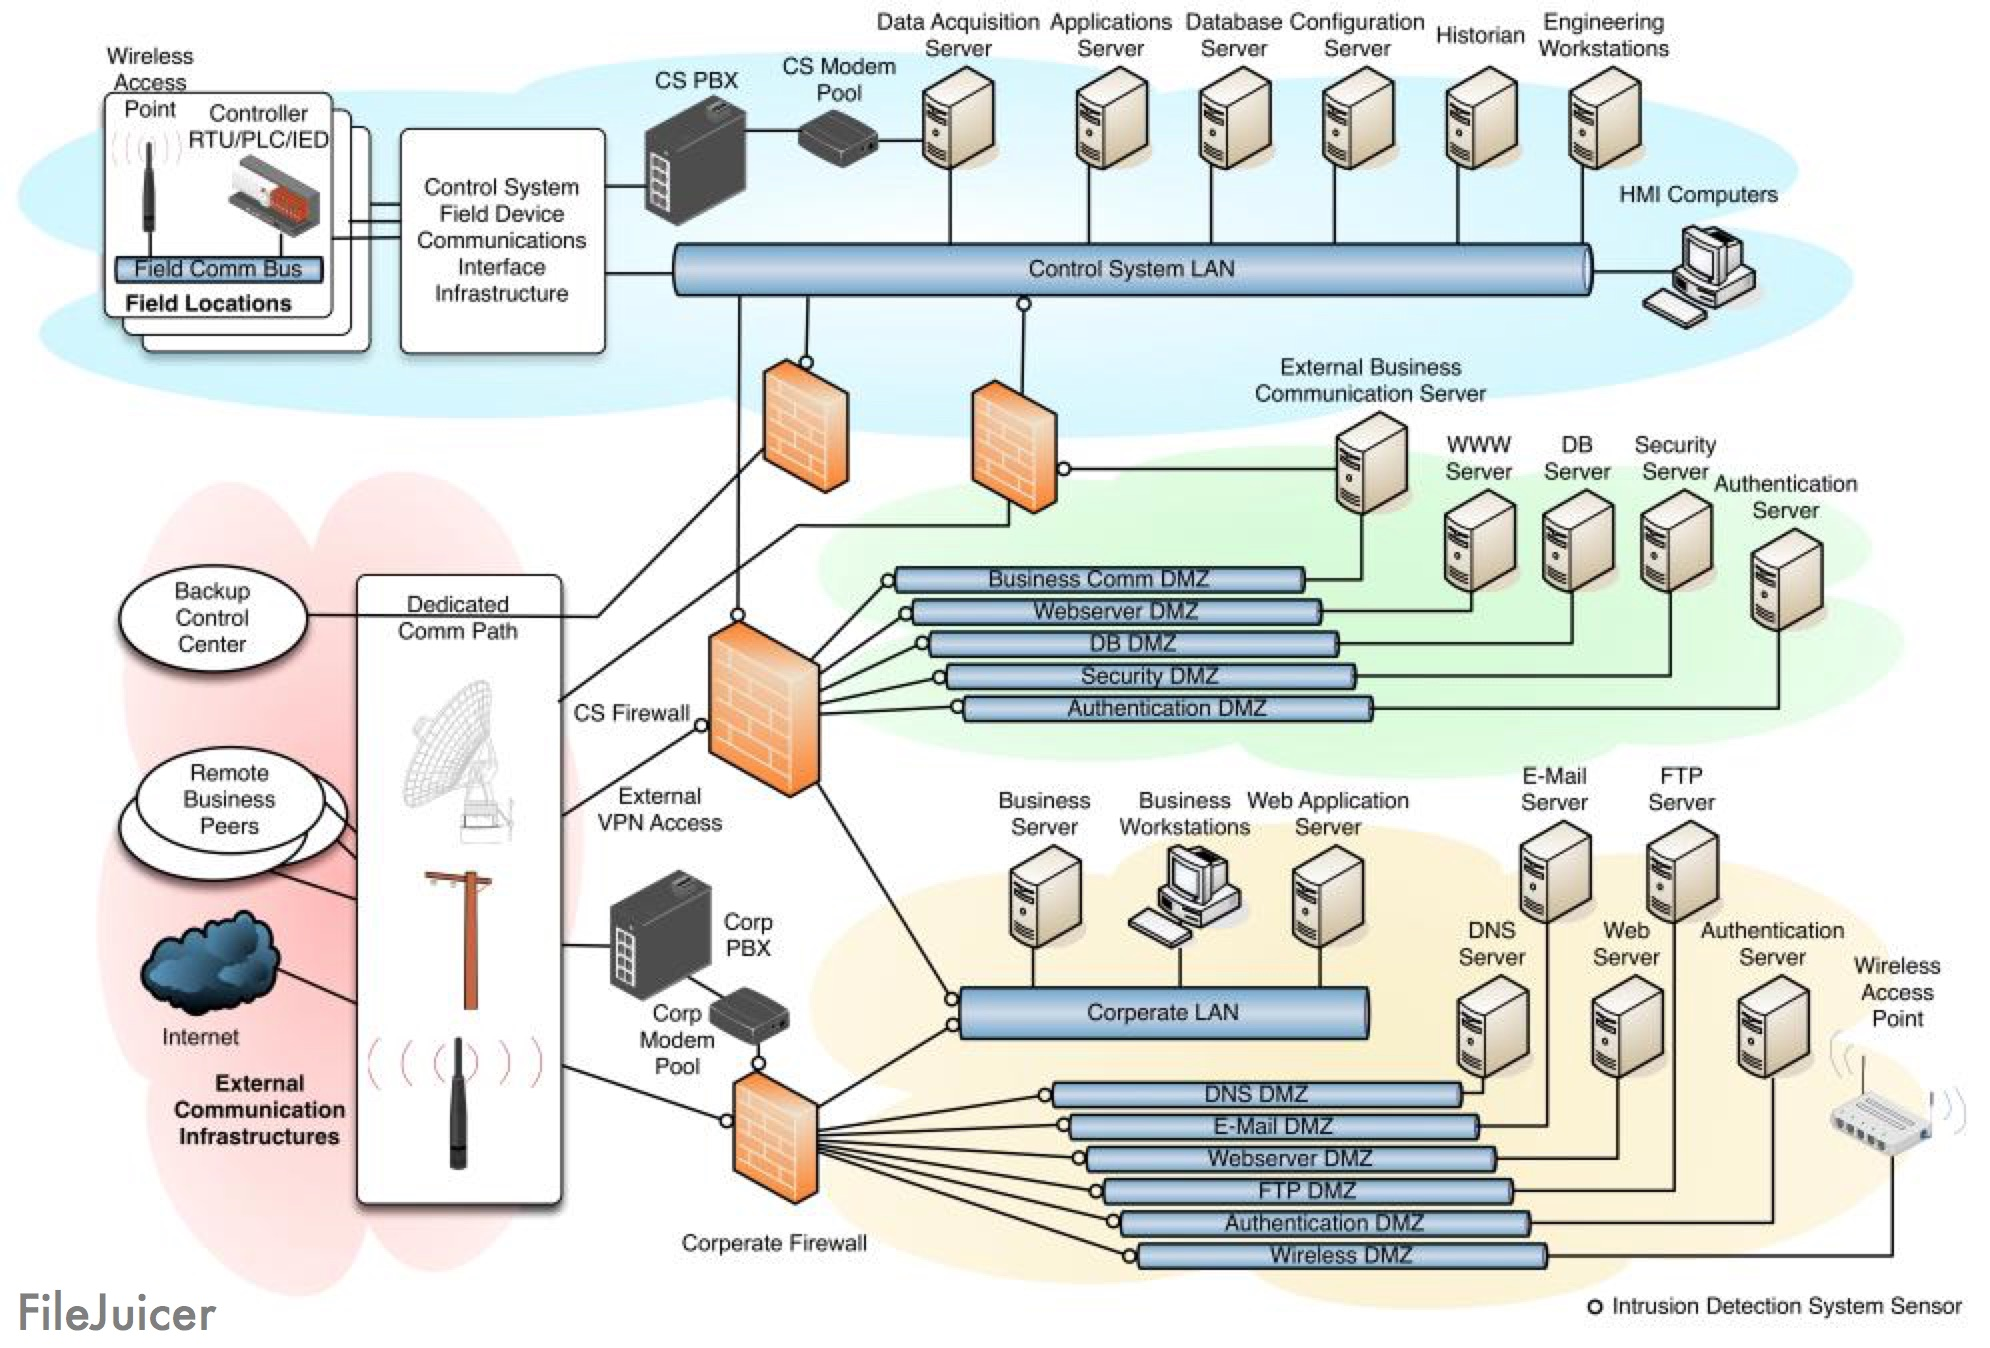
\includegraphics[width=15cm]{defense-in-depth-strategie}
    \caption{Defense in Depth Strategie - \cite{kuipers2006}}
    \label{Kap3:Defense-in-Depth}
\end{figure}

\clearpage

Das Defense in Depth Konzept stellt ein Konzept dar, um Industrieanlagen und Unternehmensnetzwerke vor Angriffen zu schützen. Bei der sich ständig ändernden Bedrohungslage in den komplexen Netzen wird bei dieser Strategie jedoch weniger ein vollständiger Schutz bereitgestellt, als eine Strategie zur Schadensbegrenzung im Falle eines Angriffs.